\section{ZK-ZKVM} \label{sec:zk-zkvm}

A ZK-VM \ref{sec:ola-vm} which is a system that uses zk technology to implement a verifiable circuit system for general computation. However, it has some issues where privacy is required, for example, quotation data of commercial competition, anonymous auction, etc. The generation of each program's proof executed in the ZK-VM leaks the witness data, such as the name and function of the called contract, parameters, and so on.

To address this privacy concern, the ZK-ZKVM system has been developed. This system builds on top of ZK-VM but adds an extra layer of privacy by ensuring that all witness data is private and does not reveal any information. This is achieved through the use of a key system consists of different permissioned private keys and a note mechanism similar to ZCash's UTXO model.

The basic principle of ZK-ZKVM is the use of different permissioned private keys in the key system. These keys are used to encrypt and decrypt the witness data, ensuring that it remains private and secure. Additionally, the note mechanism is used to further enhance the privacy of the system. Each note represents a certain amount of value that is spendable by the recipient, and is transmitted in ciphertext. It is impossible to deduce any information about the transaction from this ciphertext.

The importance of ZK-ZKVM lies in its ability to address the privacy concerns that exist in ZK-VM. With ZK-ZKVM, users can conduct transactions on public blockchains with the assurance that their sensitive information is secure and private. This makes it suitable for a wide range of use cases that require high levels of privacy, such as financial transactions or data sharing.

Furthermore, ZK-ZKVM also offers the same scalability benefits as ZK-VM. By allowing for off-chain computation and verification, it reduces the burden on the main blockchain and increases transaction throughput. This makes it a more efficient and effective solution for blockchain scaling than traditional solutions.

In Section \ref{section: zk-zkvm-keys-addresses}, we provide an in-depth explanation of the key system design in our ZK-ZKVM system. In the following section, Section \ref{section: zk-zkvm-notes}, we explore the note design within our ZK-ZKVM system. Moving on, in Sections \ref{section: zk-zkvm-user-end-prove} and \ref{section: zk-zkvm-delegable-prove}, we conduct a comparative analysis of two distinct approaches to proof generation. Finally, in Section \ref{section: zk-zkvm-framework}, we present the fundamental framework of ZK-ZKVM.

\subsection{Keys and Addresses}\label{section: zk-zkvm-keys-addresses}

Encryption schemes and signature schemes in cryptography are the basis for achieving privacy. Encryption schemes include symmetric encryption and asymmetric encryption. In symmetric encryption, the sender and recipient first agree with a secret between them using key agreement scheme, and then derive a symmetric key from the secret for encryption and decryption. In asymmetric encryption, the sender encrypts the plaintext with the recipient's public key, and then the recipient decrypts the ciphertext with his own private key. The signature scheme is just the opposite, the sender signs plaintext with his own private key, and others can use the sender's public key to verify the signature.

A variety of encryption and signature schemes are used in Ola to protect privacy. At the same time, in order to enable the separation of spending and viewing permissions, some new keys are derived based on the elliptic curve algorithm, which constitutes Ola's key system.

\begin{figure}[!htp]
    \centering
    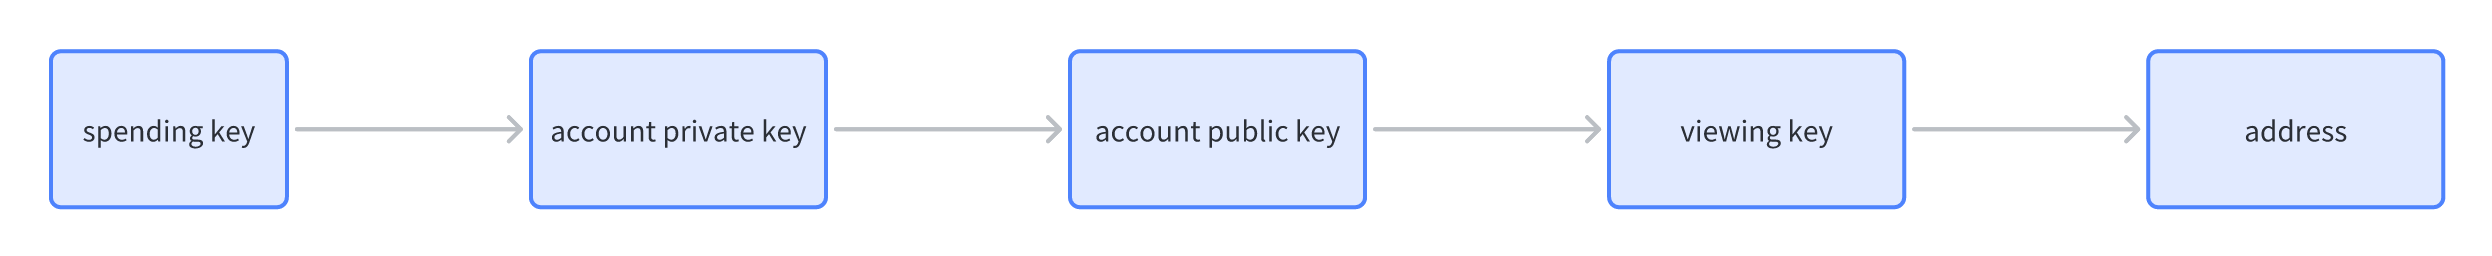
\includegraphics[width=0.8\textwidth]{key_system.png}
    \caption{Key system of Ola}
    \label{fig: key_system}
\end{figure}

\subsubsection{Spending Keys}\label{section: spending-keys}

Spending keys are the most important keys in the key system. Similar to the private keys in Bitcoin, whoever owns the spending key can spend and view the balance and transaction history in the address associated with this key. The Spending key is used to generate other keys, which is essentially a 256-bit random number, which makes it as secure as Bitcoin in some respects.
\subsubsection{Account Private Keys}\label{section: account-private-keys}

Account private keys are derived from the associated spending keys. Account private keys are private keys just like the spending keys and can not be leaked to others. A Account private key can be used to sign transactions and generate note commitments. It mainly consists of three parts:

\begin{itemize}
    \item Random commitment key
        \begin{itemize}
            \item a random number used in commitment scheme
        \end{itemize}
    \item Signature secret key
        \begin{itemize}
            \item A key used in signature scheme
        \end{itemize}
    \item Random seed
        \begin{itemize}
            \item A random number seed
            \item Signature secret key and rcm are all derived from a rseed
        \end{itemize}
\end{itemize}

The random commitment key is a scalar used in commitment schemes. The signature secret key is also a scalar used for private keys in signature schemes. The random seed is a random number generated by a random number generator, which is an element in a finite field and is 32 bytes in size.
\subsubsection{Account Public Keys}\label{section: account-public-keys}

Account public keys are derived from the associated account private keys, which mainly includes:

\begin{itemize}
    \item Signature public key
    \item Signature public random key
    \item PRF secret key
\end{itemize}

The signature public key is a public key derived from the generator G of the group on an elliptic curve and a signature secret key, which is essentially a group element on the elliptic curve, and is used to verify the signature in a signature scheme
\[ \mathrm{Sig\_Pub\_Key} = G^{\mathrm{Sig\_Pri\_Key}} \]

The signature public random key is a random number derived from random commitment key for a signature scheme, and is essentially an element of the group defined on the elliptic curve
\[ \mathrm{Sig\_Pub\_Rand} = G^{\mathrm{rcm}} \]

The PRF secret key is a key used in the Pseudo Random Function to generate pseudo-random numbers
\[ \mathrm{PRF}_{sk}(x) = \mathrm{Hash}(sk \mathbin{||} x) \]

\subsubsection{Viewing Keys}\label{section: viewing-keys}

Viewing keys are derived from associated account private keys, and each viewing key can generate one or more addresses. A viewing key can decrypt all transaction records associated with its address, that is, arbitrarily read transaction data under the address, so they can be used by regulatory departments to audit the historical transactions of an account. It can also be handed over to an delegate to generate zero-knowledge proofs. After the viewing key is leaked, all transaction data will be traced, but no assets will be lost (only the account private key can spend the user's assets). Viewing keys can only be issued to trusted institutions.

The viewing key is derived directly from the user's account private key
$$viewing\_key = private\_key.sk + private\_key.rcm + public\_key.sk\_prf$$

The main reason for creating a viewing key is to separate spending permissions and viewing permissions for user addresses. Users can share the viewing key with others to help themselves when necessary (such as asking delegates to generate zero-knowledge proofs for themselves), while keeping the spend key private.
\subsubsection{Addresses}\label{section: addresses}

Addresses are generated by associated account public keys or viewing keys to receive transfers. Addresses in Ola are either transparent or shielded (private). Transparent addresses are publicly visible on the blockchain, in the same way that Bitcoin addresses are viewable. Shielded addresses are invisible and transactions between shielded addresses do not reveal either address, the transaction value or the content of the encrypted field.

Zcash has defined a mechanism for generating hierarchical deterministic wallets in \href{https://zips.z.cash/zip-0032}{ZIP 32}, just like \href{https://github.com/bitcoin/bips/blob/master/bip-0032.mediawiki}{BIP 32}. It can help users who want to generate multiple addresses per account. All derivations produce an opaque binary spending key, from which the keys and addresses are then derived.

\begin{itemize}
    \item ZIP 32
        \begin{itemize}
            \item Account 0
                \begin{itemize}
                    \item Diversified address 0
                    \item Diversified address 1
                    \item ...
                \end{itemize}
            \item Account 1
                \begin{itemize}
                    \item Diversified address 0
                    \item Diversified address 1
                    \item ...
                \end{itemize}
            \item ...
        \end{itemize}
\end{itemize}

Ola will also design a similar mechanism in the future to implement a lightweight diversified address derivation scheme, which provides different payment addresses to different senders when users receive money to better protect the privacy of users.
\subsection{Notes}\label{section: zk-zkvm-notes}

\subsubsection{Introduction}\label{section: note-introduction}

There are mainly two storage models in blockchain:  the UTXO model used by Bitcoin and the account model use by Ethereum. UTXO is the abbreviation of Unspent Transaction Outputs, it mainly focuses on the equality of input and output. Transferring or updating contract status in the UTXO model performs consuming old notes and producing new notes. The account model, on the contrary, focuses on data such as the balance of the account stored in a location associated with the account. Transferring or updating the contract state can directly modify the data in the same location. Ola uses the UTXO model to implement a private account system, and also supports the account model to implement a public accounts system.

The main reasons why the private account system is implemented using the UTXO model rather than directly based on the account model are:

\begin{enumerate}
    \item Account model updates directly update the state in the location of the account, which makes it easy to leak user identity information.
    \item The account model supports privacy requires updating states of all users and contracts at the same time, which is less efficient.
    \item UTXO model can address the above two problems and enables efficient implementation of privacy features.
\end{enumerate}

In the private account system, a user's balance information and state data are stored in a data structure called Note (refer to Zcash). A note mainly contains:

\begin{itemize}
    \item Spend public key
        \begin{itemize}
            \item The public key of the owner of the note, that is, the holder of the private key corresponding to this public key can consume this note.
        \end{itemize}
    \item Amount
        \begin{itemize}
            \item The amount of tokens in the note, that is, the value that this note can spend.
        \end{itemize}
    \item Payload
        \begin{itemize}
            \item Data stored in this note.
        \end{itemize}
    \item Birth predicate
        \begin{itemize}
            \item Conditions that need to be met to create this note.
        \end{itemize}
    \item Death predicate
        \begin{itemize}
            \item Conditions that need to be met to consume this note.
        \end{itemize}
    \item Random commitment key
        \begin{itemize}
            \item Used to generate note commitment corresponding to this note.
        \end{itemize}
    \item Nullifier key
        \begin{itemize}
            \item Used to generate nullifier corresponding to this note.
        \end{itemize}
\end{itemize}

The above note is represented by the vector group, which can be expressed as: 
(spend public key, amount, payload, birth, death, random commitment key, nullifier key).
\subsubsection{Note Commitments and Nullifiers}\label{section: commitments-nullifiers}

When each note is created, a corresponding note commitment is generated, and the note commitment promises the validity of all parameters in the note.
\[ \text{note\_commitment} = \text{Commit}(\text{note})\]

Note commitments and notes have a one-to-one bijection relationship, that is, there are no two different notes with the same note commitment, and vice versa. Unlike the account model, there is not a Merkle tree on the chain to store all states, but the ciphertext of notes is scattered among transactions in all blocks, and sequencers only maintain a notes commitment tree. When creating a note, users need to prove that the note commitment of this new note is on the current merkle tree through a zero-knowledge proof.

Every note has a nullifier, generated by the nullifier key and note commitment. In addition to the note commitment tree, sequencers also maintain a nullifier set. When a note is spent, the nullifier of the note needs to be revealed publicly. The node needs to check that the nullifier is not added to the nullifier set, otherwise it will cause the double spending problem.
\[ \text{nullifier} = \mathrm{Hash}(\text{nullifier\_key} \mathbin{||} \text{note\_commitment}) \]

\subsubsection{Send notes}\label{section: send-notes}

In order to protect user privacy, the notes in the ledger can not be updated once they are generated. Instead, old notes need to be marked as spent by revealing their nullifiers, and produce new notes and append them to the ledger.
After the user selects old notes and produces new notes, they need to encapsulate the note ciphertexts into a transaction and submit it to a sequencer. There are some other fields in the transaction, such as an aggregated zero-knowledge proof. The process of sending notes is as follows:

\begin{enumerate}
    \item Select the notes to be spent and the recipient's shielded address.
    \begin{enumerate}
        \item A shielded address contains a public key called spending public key.
    \end{enumerate}
    \item Decrypt the note ciphertexts to get note plaintexts of the selected old notes.
    \item Get the random commitment keys and the nullifier keys of old notes from their plaintexts.
    \item Generate note commitments of old notes using the random commitment keys.
    \item Generate proofs of the existence of old notes on the merkle tree.
    \item Generate nullifiers of old notes through their nullifier keys.
    \item Generate an ephemeral key pair, which consists of an ephemeral private key and an ephemeral public key.
    \item Use the spending public key and the ephemeral private key as inputs of the key agreement scheme to generate a shared secret.
    \item Derive a symmetric key sym\_key from the shared secret.
    \item Construct new note plaintexts $$np = (spending\_public\_key, value, payload, random\_commitment\_key, nullifier\_key)$$
    \item Encrypt note plaintexts using sym\_key to get note ciphertexts.
    \item Compose the above parameters into a statement.
    \item Generate a zero-knowledge proof of the statement.
    \item Assemble all old notes, new notes, the ephemeral public key and the proof into a transaction.
    \item Encode the transaction and send it to the network.
\end{enumerate}
\subsubsection{Receiving notes}\label{section: receiving-notes}

Recipients need to scan all blocks to receive notes sent to them. In each block, iterate over each transaction in it, and try to decrypt all note ciphertexts. If a note ciphertext can be decrypted by the recipient's viewing key, this means the note is sent to the recipient, and the recipient can then view the value and payload in the note and add it to his spent set. The process of scanning the blockchain is as follows:

\begin{enumerate}
    \item Enumerate every transaction in the block.
    \item Get the ephemeral public key in the transaction.
    \item Use the spending private key and the ephemeral public key as inputs to the key agreement scheme to get a shared secret.
    \item Derive a symmetric key sym\_key from the shared secret.
    \item Use sym\_key to decrypt a note ciphertext in the transaction.
    \item If decryption gets note plaintext np: 
        $$np = (\text{spending\_public\_key}, text{value}, \text{payload}, \text{random\_commitment\_key}, \text{nullifier\_key})$$
        \begin{enumerate}
            \item Generate the nullifier using nullifier\_key and random commitment key.
            \item Generate the note commitment using the random commitment key.
            \item Check if the nullifier is already in the nullifier set to prevent double spending.
            \item Check if the note commitment is in the note commitment tree.
            \item Add the valid note to a spent set.
        \end{enumerate}
    \item If it cannot be decrypted, try the next note ciphertext.
    \item Return the spent set.
\end{enumerate}

The user's balance and all on-chain state is the sum of the notes in the spent set.

\subsection{Proof Generation}\label{section: zk-zkvm-user-end-prove}

Sections \ref{section: zk-zkvm-key} and \ref{section: zk-zkvm-note} serve as core building blocks of our ZK-ZKVM system. In this section, we will explain our proof generation scheme. For a high-level overview of the system design, please refer to section \ref{section: zk-zkvm-framework}.

Proof generation is a critical component of the ZK-ZKVM platform, designed to facilitate private and efficient execution of smart contracts on the blockchain. The platform offers both public and private functions, with private functions executed and proven on the user-side, while public functions are executed and verified on blockchain nodes.

To enable this functionality, ZK-ZKVM relies on advanced cryptographic techniques such as the key system discussed in section \ref{section: zk-zkvm-key} and note design discussed in section \ref{section: zk-zkvm-note}. These tools allow users to generate compact and efficient proofs that demonstrate their authorization to execute private functions without revealing any sensitive information about those functions.

The proof generation process involves several steps. First, in a single contract function call, there may be private and public functions. The user executes and generates a set of data (including private and public inputs) for the private function, along with a callback hook for the public function. They then use this data to generate a zero-knowledge proof that demonstrates their authorization to execute the function and validates the execution.

Next, the user submits this proof, along with their public inputs, to the blockchain node for verification. The node verifies the proof using ZK-ZKVM's public parameters (referred to as the verification key in ZK-SNARKs) to ensure that the private function is executed correctly.

Once the proof is verified, the network executes any relevant public functions on behalf of the user with the provided callback hook. Throughout this process, all sensitive information about the private function remains hidden from public view, ensuring strong privacy guarantees for all parties involved. Public state information, such as Note Commitments Tree and Nullifier Set, is stored on the node side and public functions are handled on the node as well.

\textbf{Procedure}


\subsection{Delegable Proof Generation}\label{section: zk-zkvm-delegable-prove}

The Section \ref{section: zk-zkvm-user-end-prove} scheme highlights a key challenge in generating cryptographic proofs for transactions in a blockchain network. As the complexity of the transaction and the number of calls involved increases, so does the cost of creating and including the proof in the transaction. This poses a significant problem for users, particularly those using weaker devices such as mobile phones or hardware tokens.

To address this issue, a solution called Delegable Proof Generation Scheme (DPGS) has been proposed. DPGS allows users to delegate the task of generating cryptographic proofs to a third party in a privacy-preserving manner, such as a server or a more powerful device, while still maintaining the security and validity of the transaction. This means that users can conduct complex transactions without incurring the high cost of generating proofs themselves.

The key system and note design used in DPGS ensures that transactions remain private and secure, even when proof generation is delegated to a third party. The system creates notes, which represent a certain unit of state, and each note is assigned a unique key. When a user wants to send a private transaction, they create a new note with a new stealth key and send it to the receiver. To ensure that the transaction is valid, a cryptographic proof is required to show that the note has not been previously spent or duplicated.

\subsubsection{Current design}

We compared the proof generation schemes of ZCash\cite{website:zcash-nu5}, ZEXE\cite{cryptoeprint:2018/962}, VERI-ZEXE\cite{cryptoeprint:2022/802}, Aleo\cite{website:aleo-vm}, Aztec3\cite{website:Aztec3}, and Efficient Private Delegation of zkSNARK Provers\cite{website:epdzp} as shown in the figure\ref{fig:cur_proof_generation} below:
\begin{figure}[!ht]
    \centering
    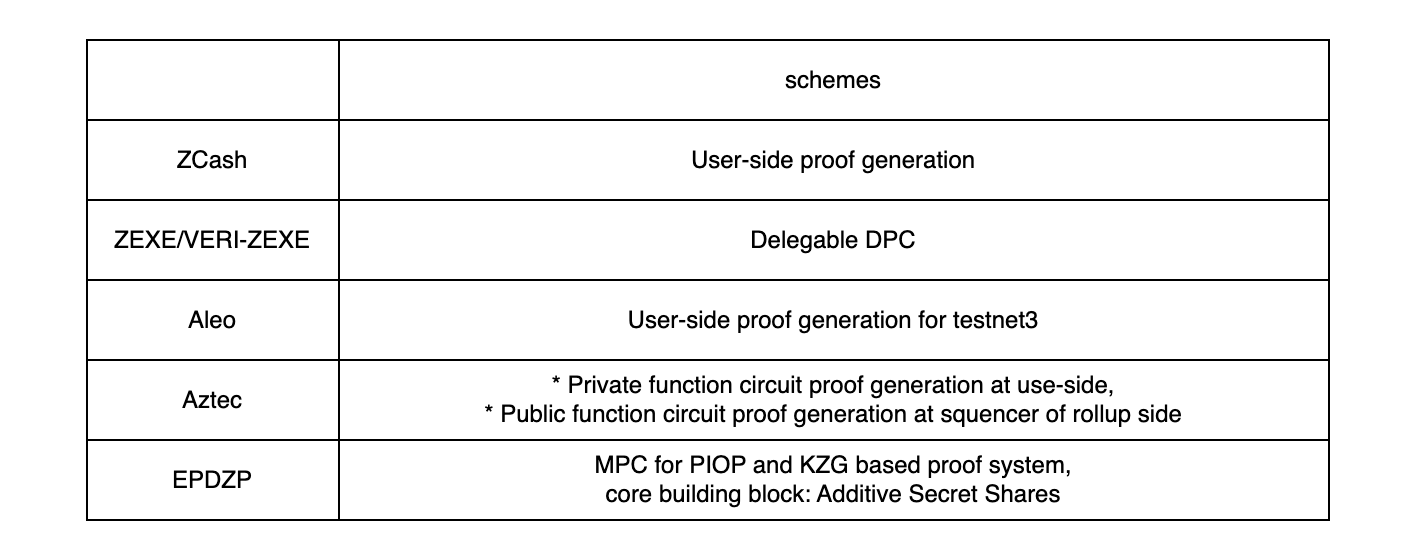
\includegraphics[width=0.6\textwidth]{cur proof generation.jpg}
    \caption{Current Proof Generation Schemes}
    \label{fig:cur_proof_generation}
\end{figure}

As we can see from above figure, ZCash's proof generation scheme is user-side proof generation, which means ZCash has only one type of transaction, which is the transfer of ZEC. The transaction is not complex and the corresponding circuit size is not very large. Therefore, when it comes to proof generation, such as for shielded transactions, it can be done on the user side, for example, generating proofs within a wallet.

The delegable DPC protocol in ZEXE\cite{cryptoeprint:2018/962} allows for the delegation of computations while maintaining security. The protocol involves a delegator who sends input parameters to a delegatee, who then performs an offline computation and generates a proof of correctness using zero-knowledge proofs. The delegatee sends this proof along with the output of the computation back to the delegator, who can use it to generate a transaction that attests to the correctness of the computation. This transaction can be publicly verified by anyone without revealing any additional information about it.

To ensure privacy, ZEXE uses a combination of cryptographic techniques such as zero-knowledge proofs and randomizable signatures. The randomizable signature scheme is used to prevent linking across multiple signatures, which is important for maintaining security in the delegable DPC protocol that the delegatee can not impersonate the delegator, e.g., by producing further transactions that the delegator never authorized.

VERI-ZEXE and ZEXE use the same delegable DPC scheme, we will not repeat it. Aleo's current implementation (testnet3) is still user-side and uses SNARK-powered circuits to generate proofs, but does not yet implement delegable DPC.

Aztec3\cite{website:Aztec3} uses a recursive circuit to generate the final proof, and each contract function is a circuit when a proof needs to be generated. The recursion uses two system circuits, private kernel circuits and public kernel circuits. All private related function calls and their proofs must be entered into private kernel circuits to generate proofs, while all public related function calls and their proofs must be entered into public kernel circuits to generate proofs. In short, the proof of the private circuit is generated on the client side, while the proof of the public circuit is generated in Rollup's Squencer.

Efficient Private Delegation of zkSNARK Provers\cite{website:epdzp} uses MPC to do outsouring proveing. While it keeps witness private and proving efficient, it is designed for Polynomial IOPs and MPC friendly polynomial commitments proof system, while our ZK-ZKVM uses Starky as its internal proof system, which is not suitable for it.

\subsubsection{Our work}

Our design based on ZEXE, and the main procedure of delegable transactions as shown in the figure\ref{fig:delegable_tx} below:

\begin{figure}[!ht]
    \centering
    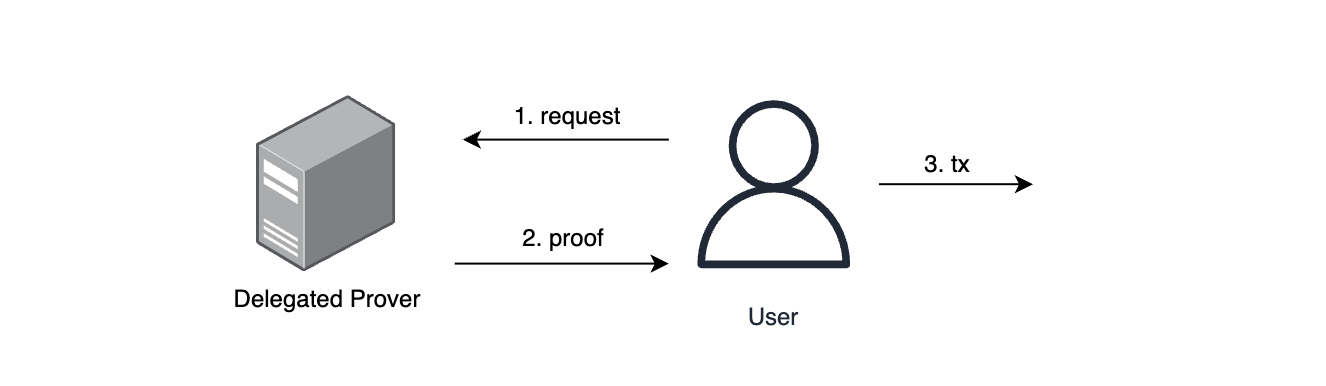
\includegraphics[width=0.6\textwidth]{delegable tx.jpg}
    \caption{Delegable transactions}
    \label{fig:delegable_tx}
\end{figure}

Although ZEXE does not allow the delegatee to impersonate the delegator, the witness remains visible to all participants on the public blockchain. This lack of privacy does not serve our purpose for ZK-ZKVM. To address this issue, we incorporated an external cryptographic primitive called the Secret Share Scheme.

We generate a shared secret by combining the delegatee's public key with the delegator's private key. We then use this shared key to symmetrically encrypt the witness on the delegator's side, and send the encrypted witness to the delegatee. The delegatee uses their private key and the delegator's public key to retrieve the shared key and decrypt the witness.

Once the witness data is decrypted, the subsequent process is identical to that of ZEXE.

Let's say User Alice is the delegator, Prover Bob is the delegatee. We briefly explain our delegable prove scheme:
\color{blue!50!black}
\begin{itemize}
    \item Alice generates shared key $key_{shared} = sk_{alice} \cdot pk_{bob}$
    \item Alice encrypt the witness, the encrypted witness is $witness_{enc} = enc(key_{shared}, witness)$
    \item Alice send the encrypted witness to Bob, while other participants on the public blockchain knows nothing.
    \item Bob generates shared key $key_{shared}' = sk_{bob} \cdot pk_{alice}$, which is same as $key_{shared}$
    \item Bob decrypt the encrypted witness, get raw witness, $witness = dec(key_{shared}', witness_{enc})$
    \item Bob use decrypted witness generating proof $\pi$, send proof back to Alice.
    \item Alice uses her signature private key to construct a transaction within proofs, send it to the blockchain.
\end{itemize}
\normalcolor{}

Our high-level description of our scheme as shown in the figure\ref{fig:our_proof_generation} below:
\begin{figure}[!ht]
    \centering
    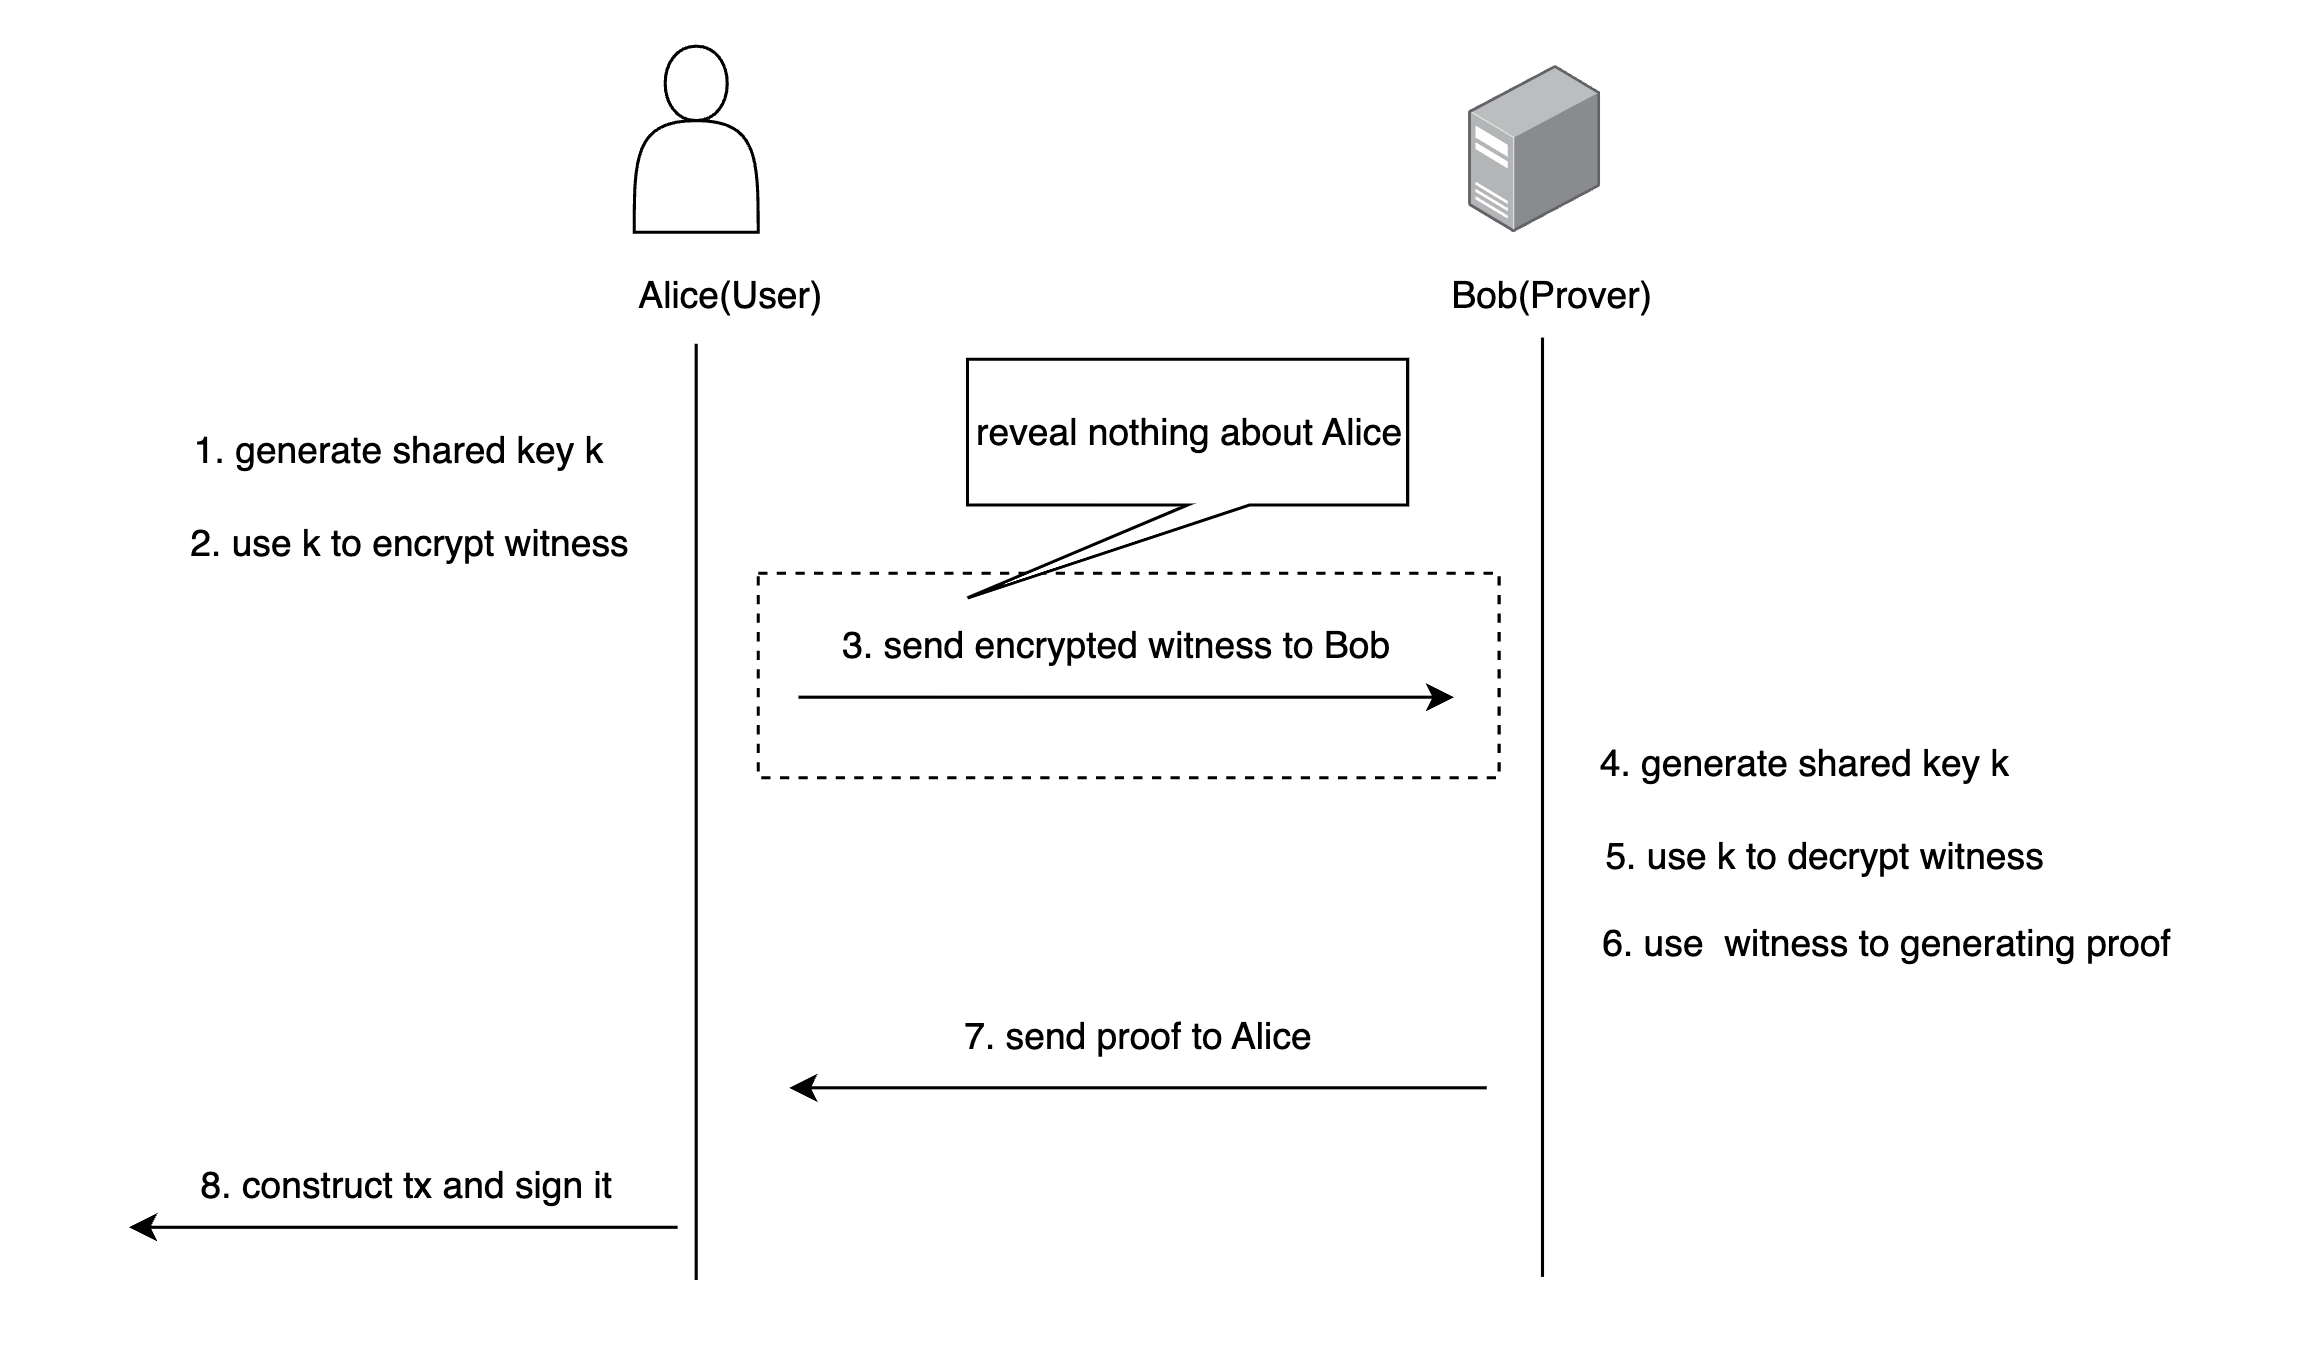
\includegraphics[width=0.6\textwidth]{our proof generation.jpg}
    \caption{Our Proof Generation Scheme}
    \label{fig:our_proof_generation}
\end{figure} 

\subsection{Framework}\label{section: zk-zkvm-framework}

The building blocks of ZK-ZKVM are:

\textbf{Key System.} Here is the summary of Key System \ref{section: zk-zkvm-key}:

\begin{itemize}
    \item The system will use a public-private key pair to enable spending and viewing of funds.
    \item The spending key will be used to sign transactions such as transfer funds.
    \item The viewing key will allow the holder to view transactions without being able to spend the funds.
    \item The system will ensure that transactions can only be signed using the correct spending key.
\end{itemize}
\bigskip

\textbf{Note Model.} Here is the summary of Note design \ref{section: zk-zkvm-note}:

\begin{itemize}
    \item The system will use a UTXO (Unspent Transaction Output) model to track the ownership of state/funds.
    \item Each private transaction will create one or more new Notes, which can be spent in future transactions.
    \item The system will ensure that transactions can only spend Notes that are owned by the signer of the transaction.
    \item The Note reveals nothing but a meaningless string to other users.
\end{itemize}
\bigskip

\textbf{Private/Public execution.} Here are the descriptions of Private/Public execution:

\begin{itemize}
    \item There are two kinds of functions for users in our system: private or public functions.
    \item Private functions have return values (AKA Notes), while public functions do not.
    \item Private functions will be executed and proved by the signer of the transaction, using Key System and Notes as core techniques described above.
    \item Private state can be decrypted by the owner's key, while it can only be spent by the spending key and is read-only when decrypted by the viewing key.
    \item Public functions have a callback hook, which is used in the Node's execution and verification phase.
    \item Private functions can call Public functions, but not the other way around.
\end{itemize}
\bigskip

\textbf{Smart Contract.} As we said in earlier Chapter \ref{sec:zk-zkvm}, this is a ZK-ZKVM, which means it supports arbitrary smart contracts.
